\vspace*{\fill}
\columnbreak

\section{Sequential Circuit Design}
\label{sec:seq-circ-design}

Sequential circuit design is to produce a working circuit for a given description or problem.

\subsection{Excitation Tables}

Excitation table is \textit{a table that lists the required inputs for a given change of state}.
\begin{figure}[H]
  \centering
  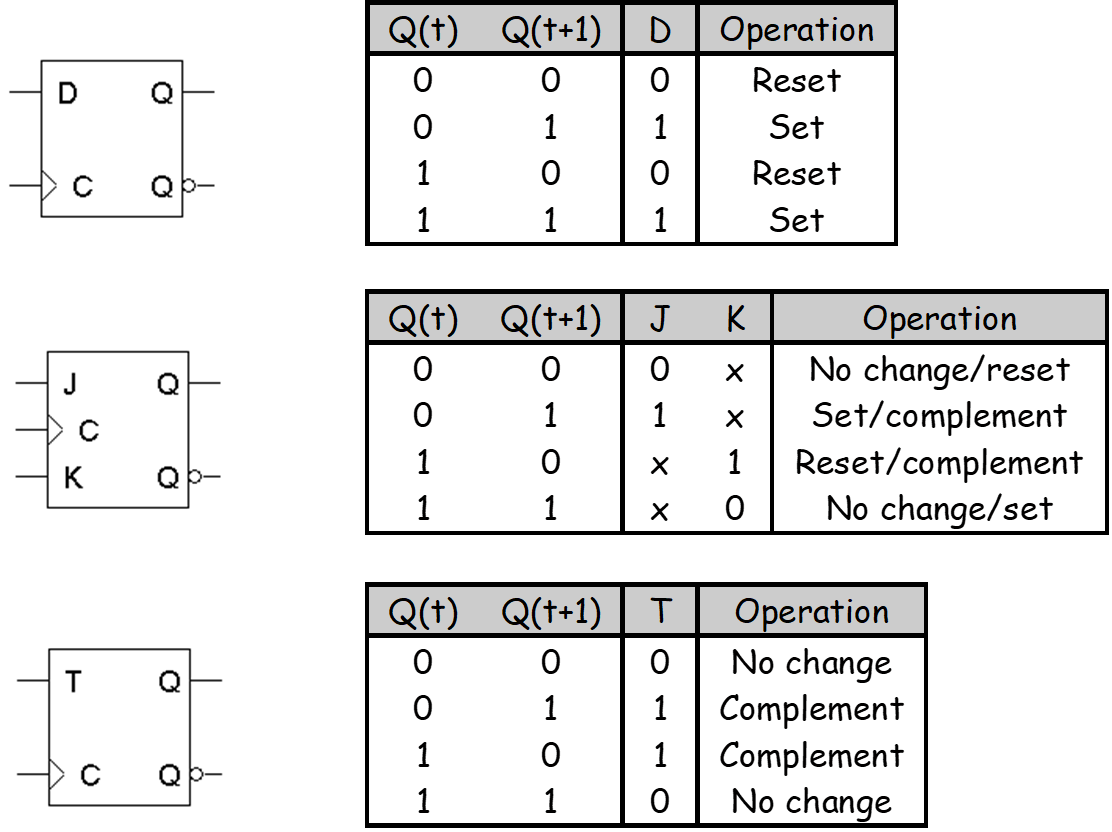
\includegraphics[width=\linewidth]{img/excitation-tables.png}
  \caption{Excitation Tables of Flip-Flops}
  \label{fig:excitation-tables}
\end{figure}

\subsection{Sequential Circuit Design Procedure}
\label{subsec:seq-circ-design-procedure}

\begin{enumerate}[label=Step\ \arabic*:, leftmargin=*]
  \item Make a state table based on the problem statement. The table should show the \textit{present states}, \textit{inputs}, \textit{next states} and \textit{outputs}. (\textit{It may be easier to find a state diagram first, and then convert that to a table.})
  \item Assign binary codes to the states in the state table (if you haven't already). If you have $n$ states, your binary codes will have at least $\lceil \log_2 n \rceil$ digits, and your circuit will have at least $\lceil \log_2 n  \rceil$ flip-flops.
  \item For each flip-flop and each row of your state table, find the flip-flop input values that are needed to generate the next state from the present state. You can use flip-flop excitation tables here.
  \item Find simplified equations for the flip-flop inputs and the outputs.
  \item Build the circuit!
\end{enumerate}

\vspace*{\fill}
\columnbreak

\subsection{Example: Sequence Recognizer}
\label{subsec:example-seq-recozginer}

Consider an example that the sequence recognizer will detect the bit pattern ``1001'' with input $X$ and output $Z$. Note that overlapping bit patterns are also detected. (1001001 will generate 0001001)

\subsubsection{Step 1: State Diagram (and Table)}
\label{subsubsec:step1-state-diagram-table}

\begin{figure}[H]
  \centering
  \begin{minipage}{\linewidth}
    \centering
    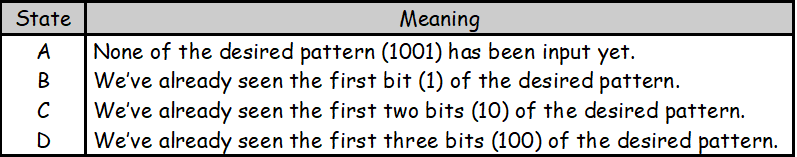
\includegraphics[width=\linewidth]{img/desing-example-table.png}
  \end{minipage}
  \begin{minipage}{\linewidth}
    \centering
    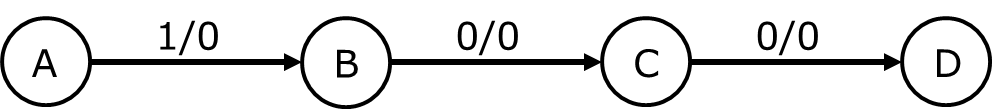
\includegraphics[width=\linewidth]{img/design-example-state-diagram.png}
  \end{minipage}
\end{figure}

What happens if we're in state D (the last three inputs were 100), and the current input is 1?
\begin{figure}[H]
  \centering
  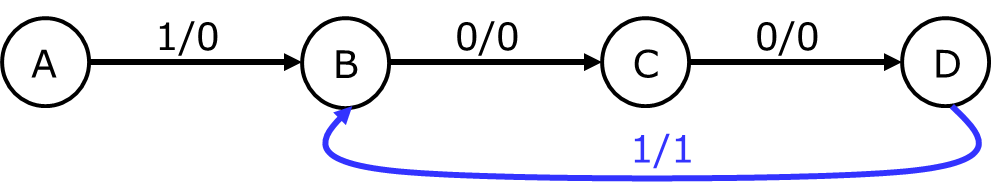
\includegraphics[width=.85\linewidth]{img/design-example-state-diagram-2.png}
\end{figure}

\noindent When we put the other arrows:
\begin{figure}[H]
  \centering
  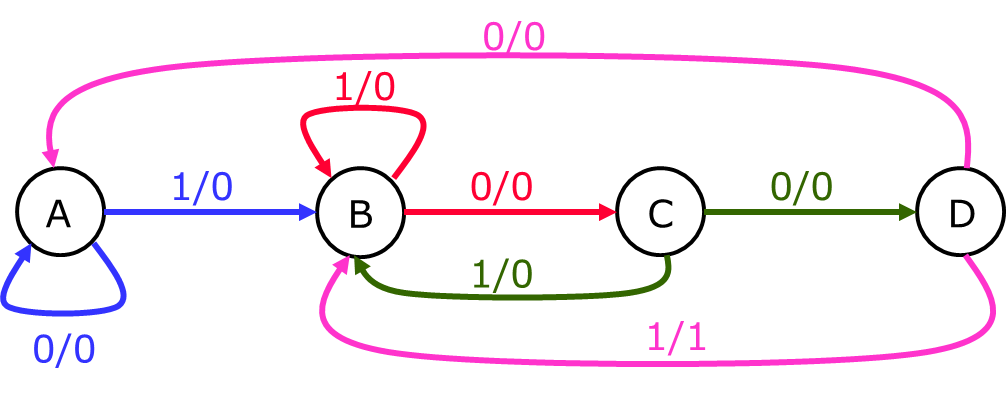
\includegraphics[width=\linewidth]{img/design-example-state-diagram-4.png}
\end{figure}
\noindent Finally, making the state table.
\begin{figure}[H]
  \centering
  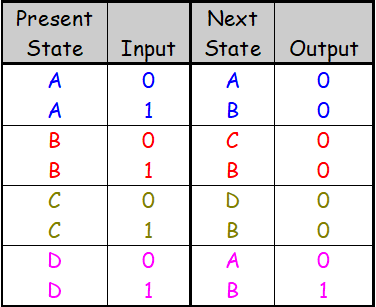
\includegraphics[width=.8\linewidth]{img/desing-example-state-table.png}
\end{figure}

\vspace*{\fill}
\columnbreak

\subsubsection{Step 2: Assigning Binary Codes}
\label{subsubsec:step2-assign-bin-code}

\begin{figure}[H]
  \centering
  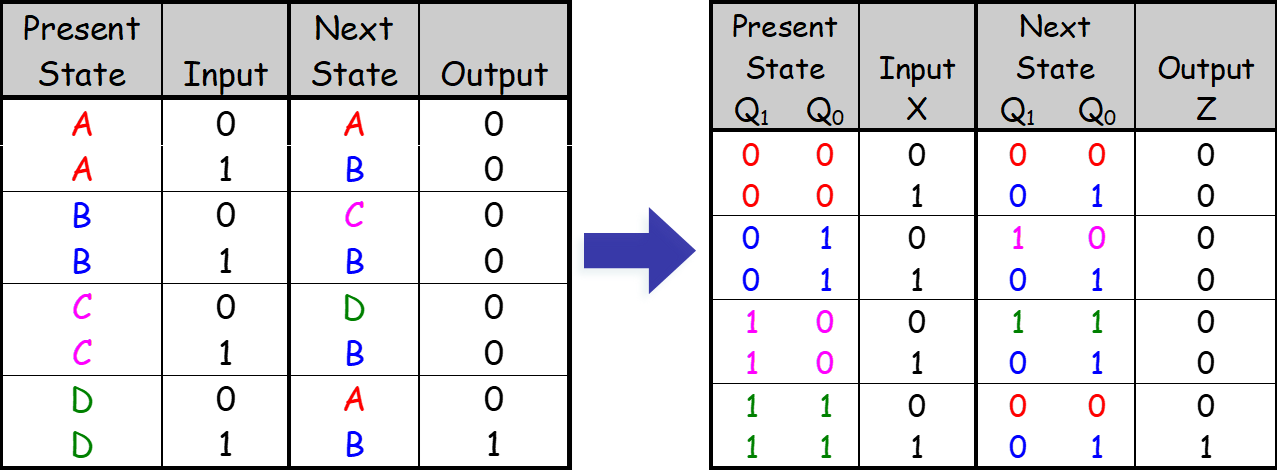
\includegraphics[width=\linewidth]{img/desing-example-state-table-2.png}
\end{figure}

\subsubsection{Step 3: Finding Flip-Flop Inputs}
\label{subsubsec:step3-finding-ff-inputs}

By using excitation table:
\begin{figure}[H]
  \centering
  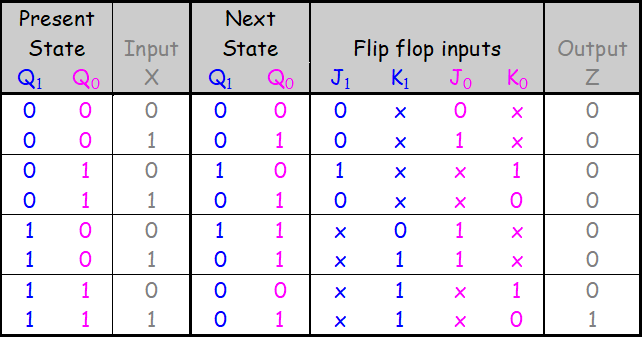
\includegraphics[width=\linewidth]{img/desing-example-state-table-3.png}
\end{figure}

\subsubsection{Step 4: Find Flip-Flop In/Out Equations}
\label{subsubsec:step4-find-ff-io-equations}

\noindent By using K-Maps, find equations for input and output:
\begin{align*}
	J_0 &= X + Q_1\\
	K_0 &= X'\\
  &\\
  J_1 &= X'Q_0\\
	K_1 &= X + Q0\\
  &\\
	Z &= Q_1Q_0X
\end{align*}

\subsubsection{Step 5: Build the Circuit}
\label{subsubsec:step5-build-the-circuit}

Lastly, we use these simplified equations to build the completed circuit.
\begin{figure}[H]
  \centering
  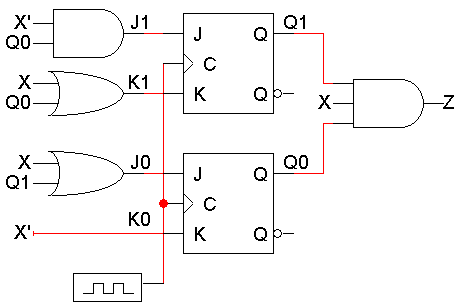
\includegraphics[width=\linewidth]{img/design-example-circuit.png}
\end{figure}